% !TeX TS-program = xelatex
% !BIB TS-program = bibtex

% Full instructions available at:
% https://github.com/pcafrica/focus-beamertheme

\documentclass{beamer}
% \usetheme{focus}
\usetheme[numbering=minimal]{focus}
% \usetheme[numbering=minimal, totalframenumbering=no]{focus}
% \usetheme[numbering=fullbar]{focus}
\definecolor{main}{RGB}{45, 45, 45}
% \definecolor{main}{HTML}{1A1A1A}
\definecolor{background}{RGB}{242, 241, 239}
% \definecolor{background}{HTML}{F5F5F5}

\usepackage{geometry}
\geometry{paperwidth=16cm, paperheight=9cm}


\title{Estimating Causal Effects Using \texorpdfstring{\\}{,} Proxy Interference Networks}
% \subtitle{Subtitle}
\author{Bar Weinstein \texorpdfstring{\\}{,} Daniel Nevo}
\titlegraphic{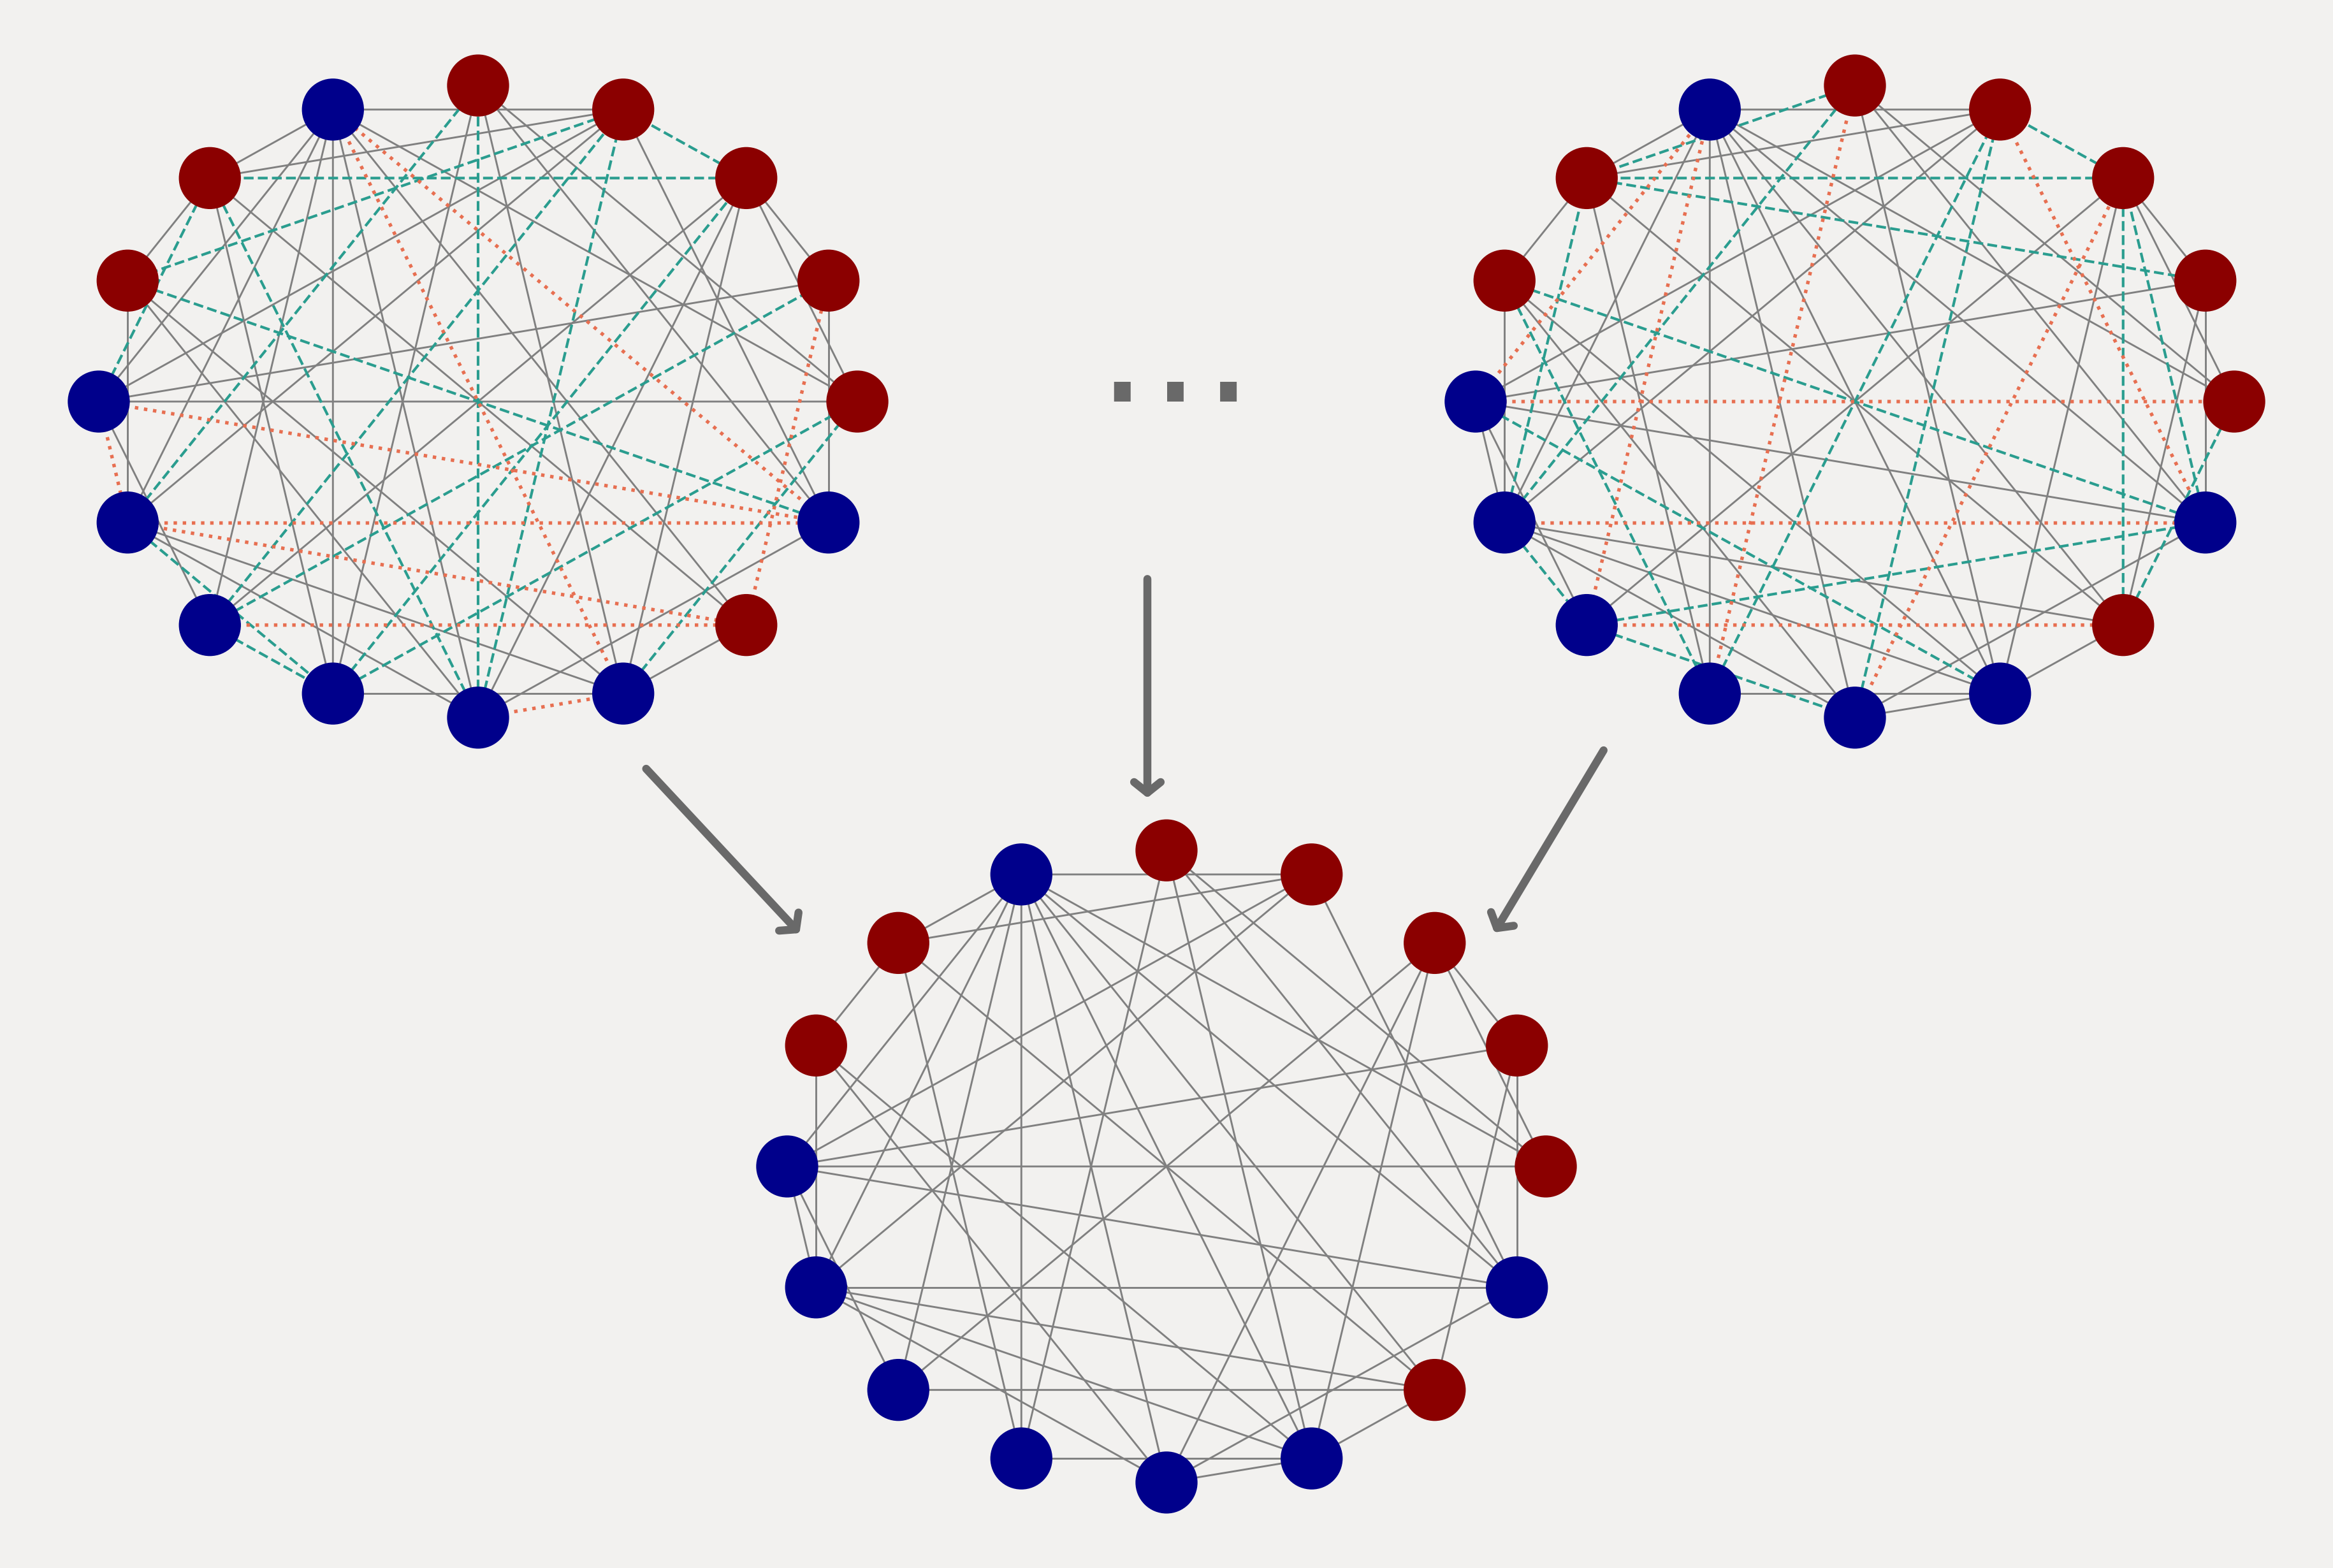
\includegraphics[scale=0.22]{figs/noisy_networks.png}}
\institute{Statistics \& OR \\ Tel Aviv University}
\date{IDSAI 2025}

% Footline info is printed only if [numbering=fullbar].
%\footlineinfo{Custom footline text}



\begin{document}
    \begin{frame}
        \maketitle
    \end{frame}
    
    % Use starred version (e.g. \section*{Section name})
    % to disable (sub)section page.
    \begin{frame}{Background}
        \large
        \begin{itemize}
            \item<1-> \textbf{Causal Inference}. Estimate the effect of treatment on an outcome. 
            \vspace{0.2cm}
            \item<1-> \textbf{Interference}. Treatment of one unit affect the outcomes of others.
            \vspace{0.2cm}
            \item<1->  Treatments spreads through a network.
            \begin{itemize}
                \item Nodes: units; Edges: magntiude of pairwise interfernce.
            \vspace{0.2cm}
            \end{itemize}
            \item<2-> Examples:
                \begin{itemize}
                    \item \emph{Social networks.} Transmission of information, behavior, encouragements, etc.
                    \vspace{0.05cm}
                    \item \emph{Epidemiology.} Mitigating spread of infectious diseases or addictive drugs.
                    \vspace{0.05cm}
                    \item A/B testing in marketplaces.
                \end{itemize} 
        \end{itemize}
    \end{frame}

    \begin{frame}[t]
        \begin{figure}[t]
            \centering
            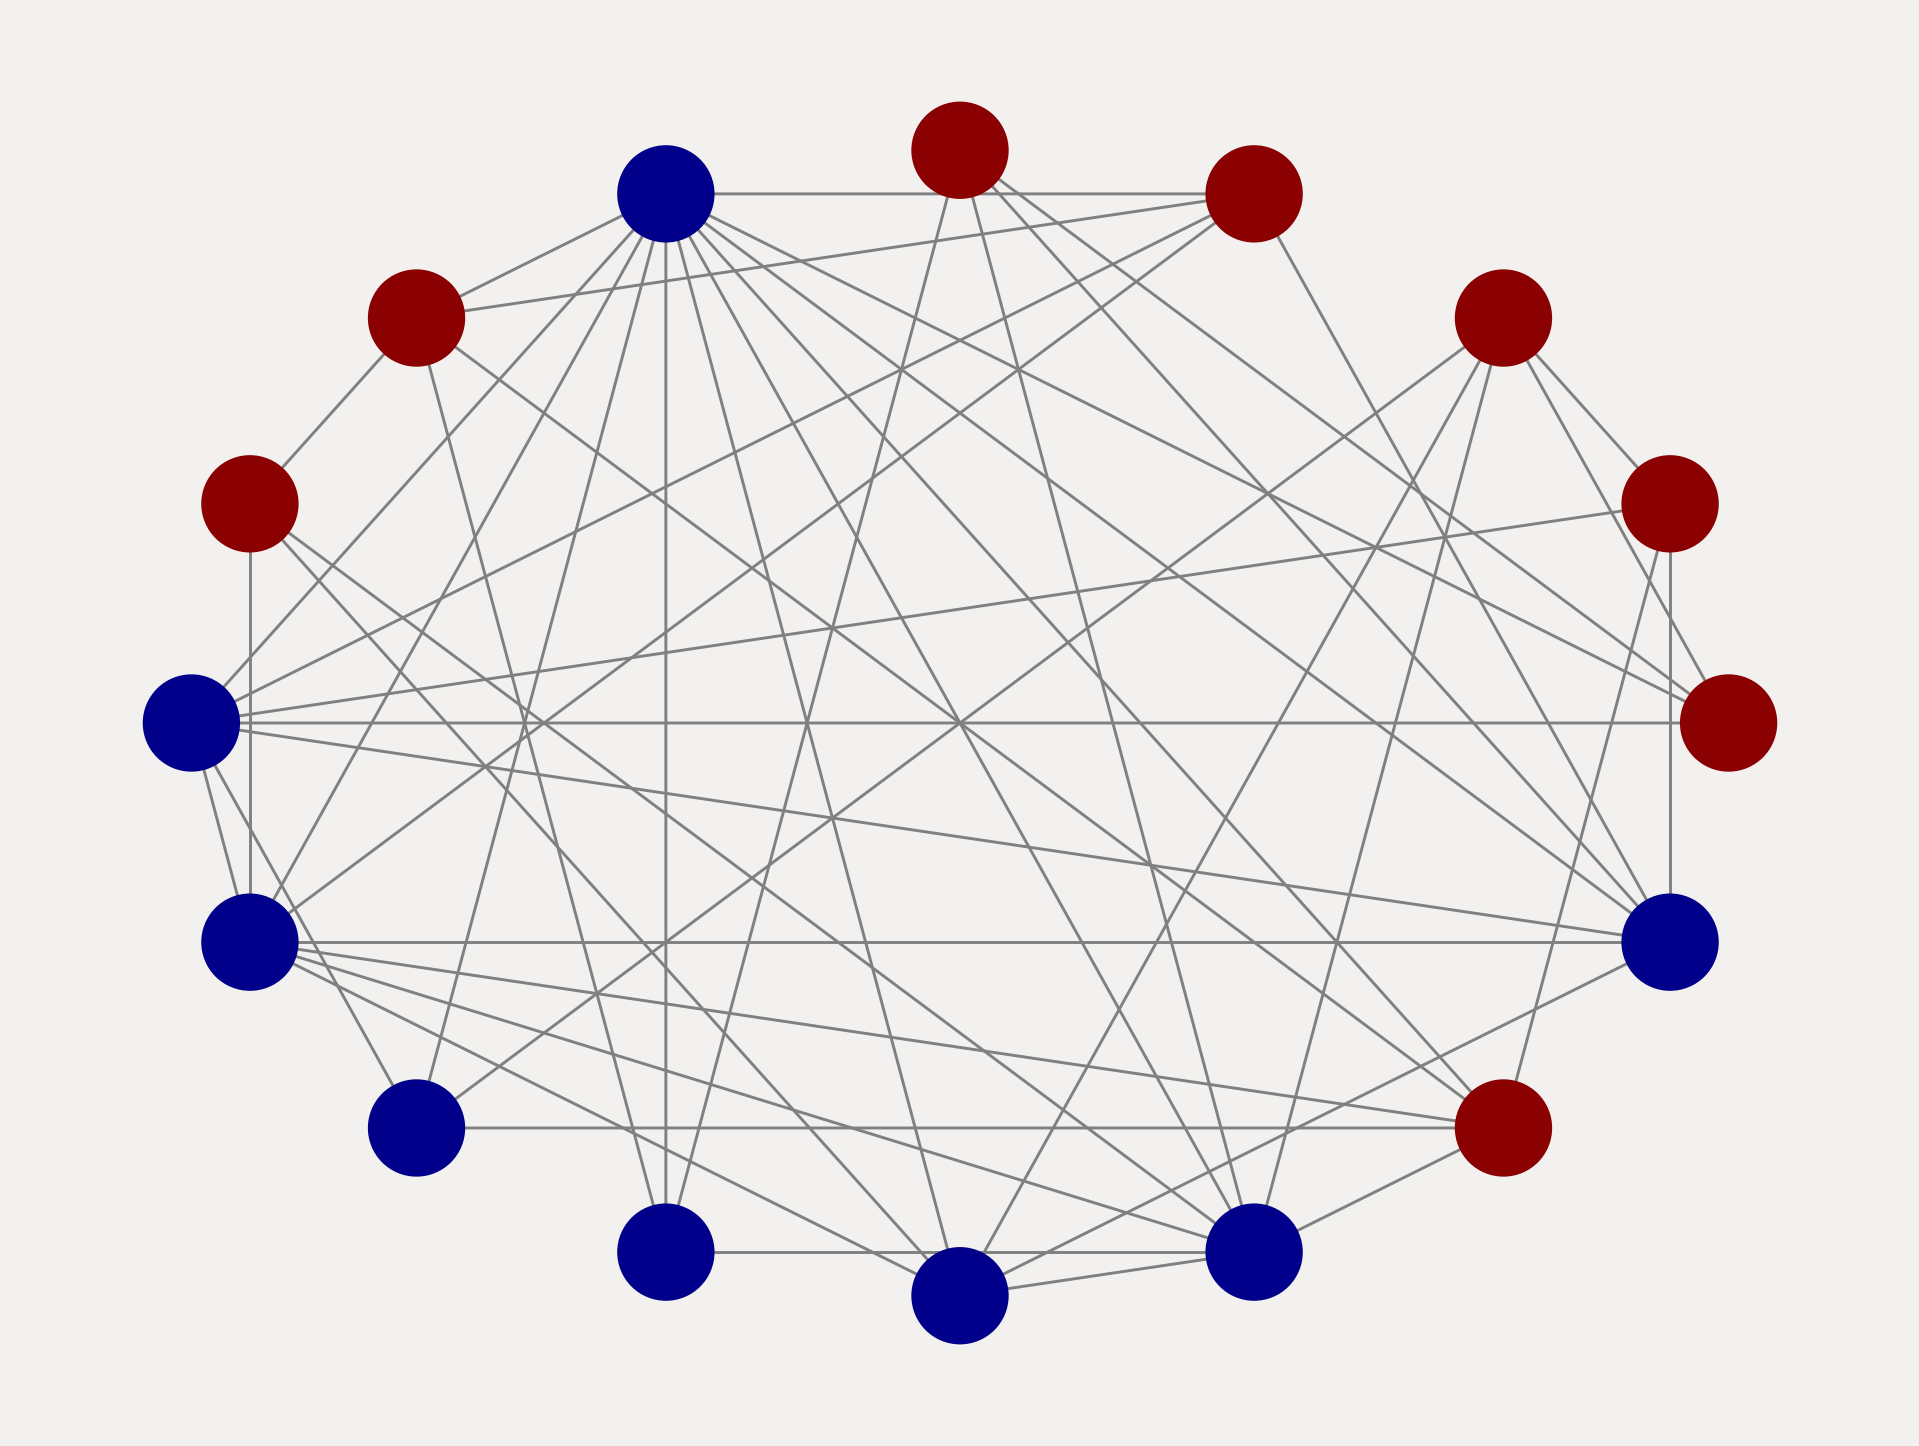
\includegraphics[width=0.65\textwidth]{figs/connected_net.png}
            % \caption{Plain frame with a figure.}
        \end{figure}
    \end{frame}

    \begin{frame}{The Challenge}
        \large
        \begin{itemize}
            \item<1-> Accurately measuring social networks is challenging.
            \vspace{0.2cm}
            \item<1-> We observe only proxy measurements of the true network.
            \begin{itemize}
                \item Measurements error.
                \item Multiple sources of data.
                \item Multilayer networks.
            \end{itemize}
            \vspace{0.2cm}
            \item<1-> True network remains latent.
        \end{itemize}
        \vspace{.5cm}
        \begin{center}
            \Large
            \textbf{How can we estimate causal effects using proxy networks?}
        \end{center}
    \end{frame}

    \begin{frame}[t]
        \begin{figure}[t]
            \centering
            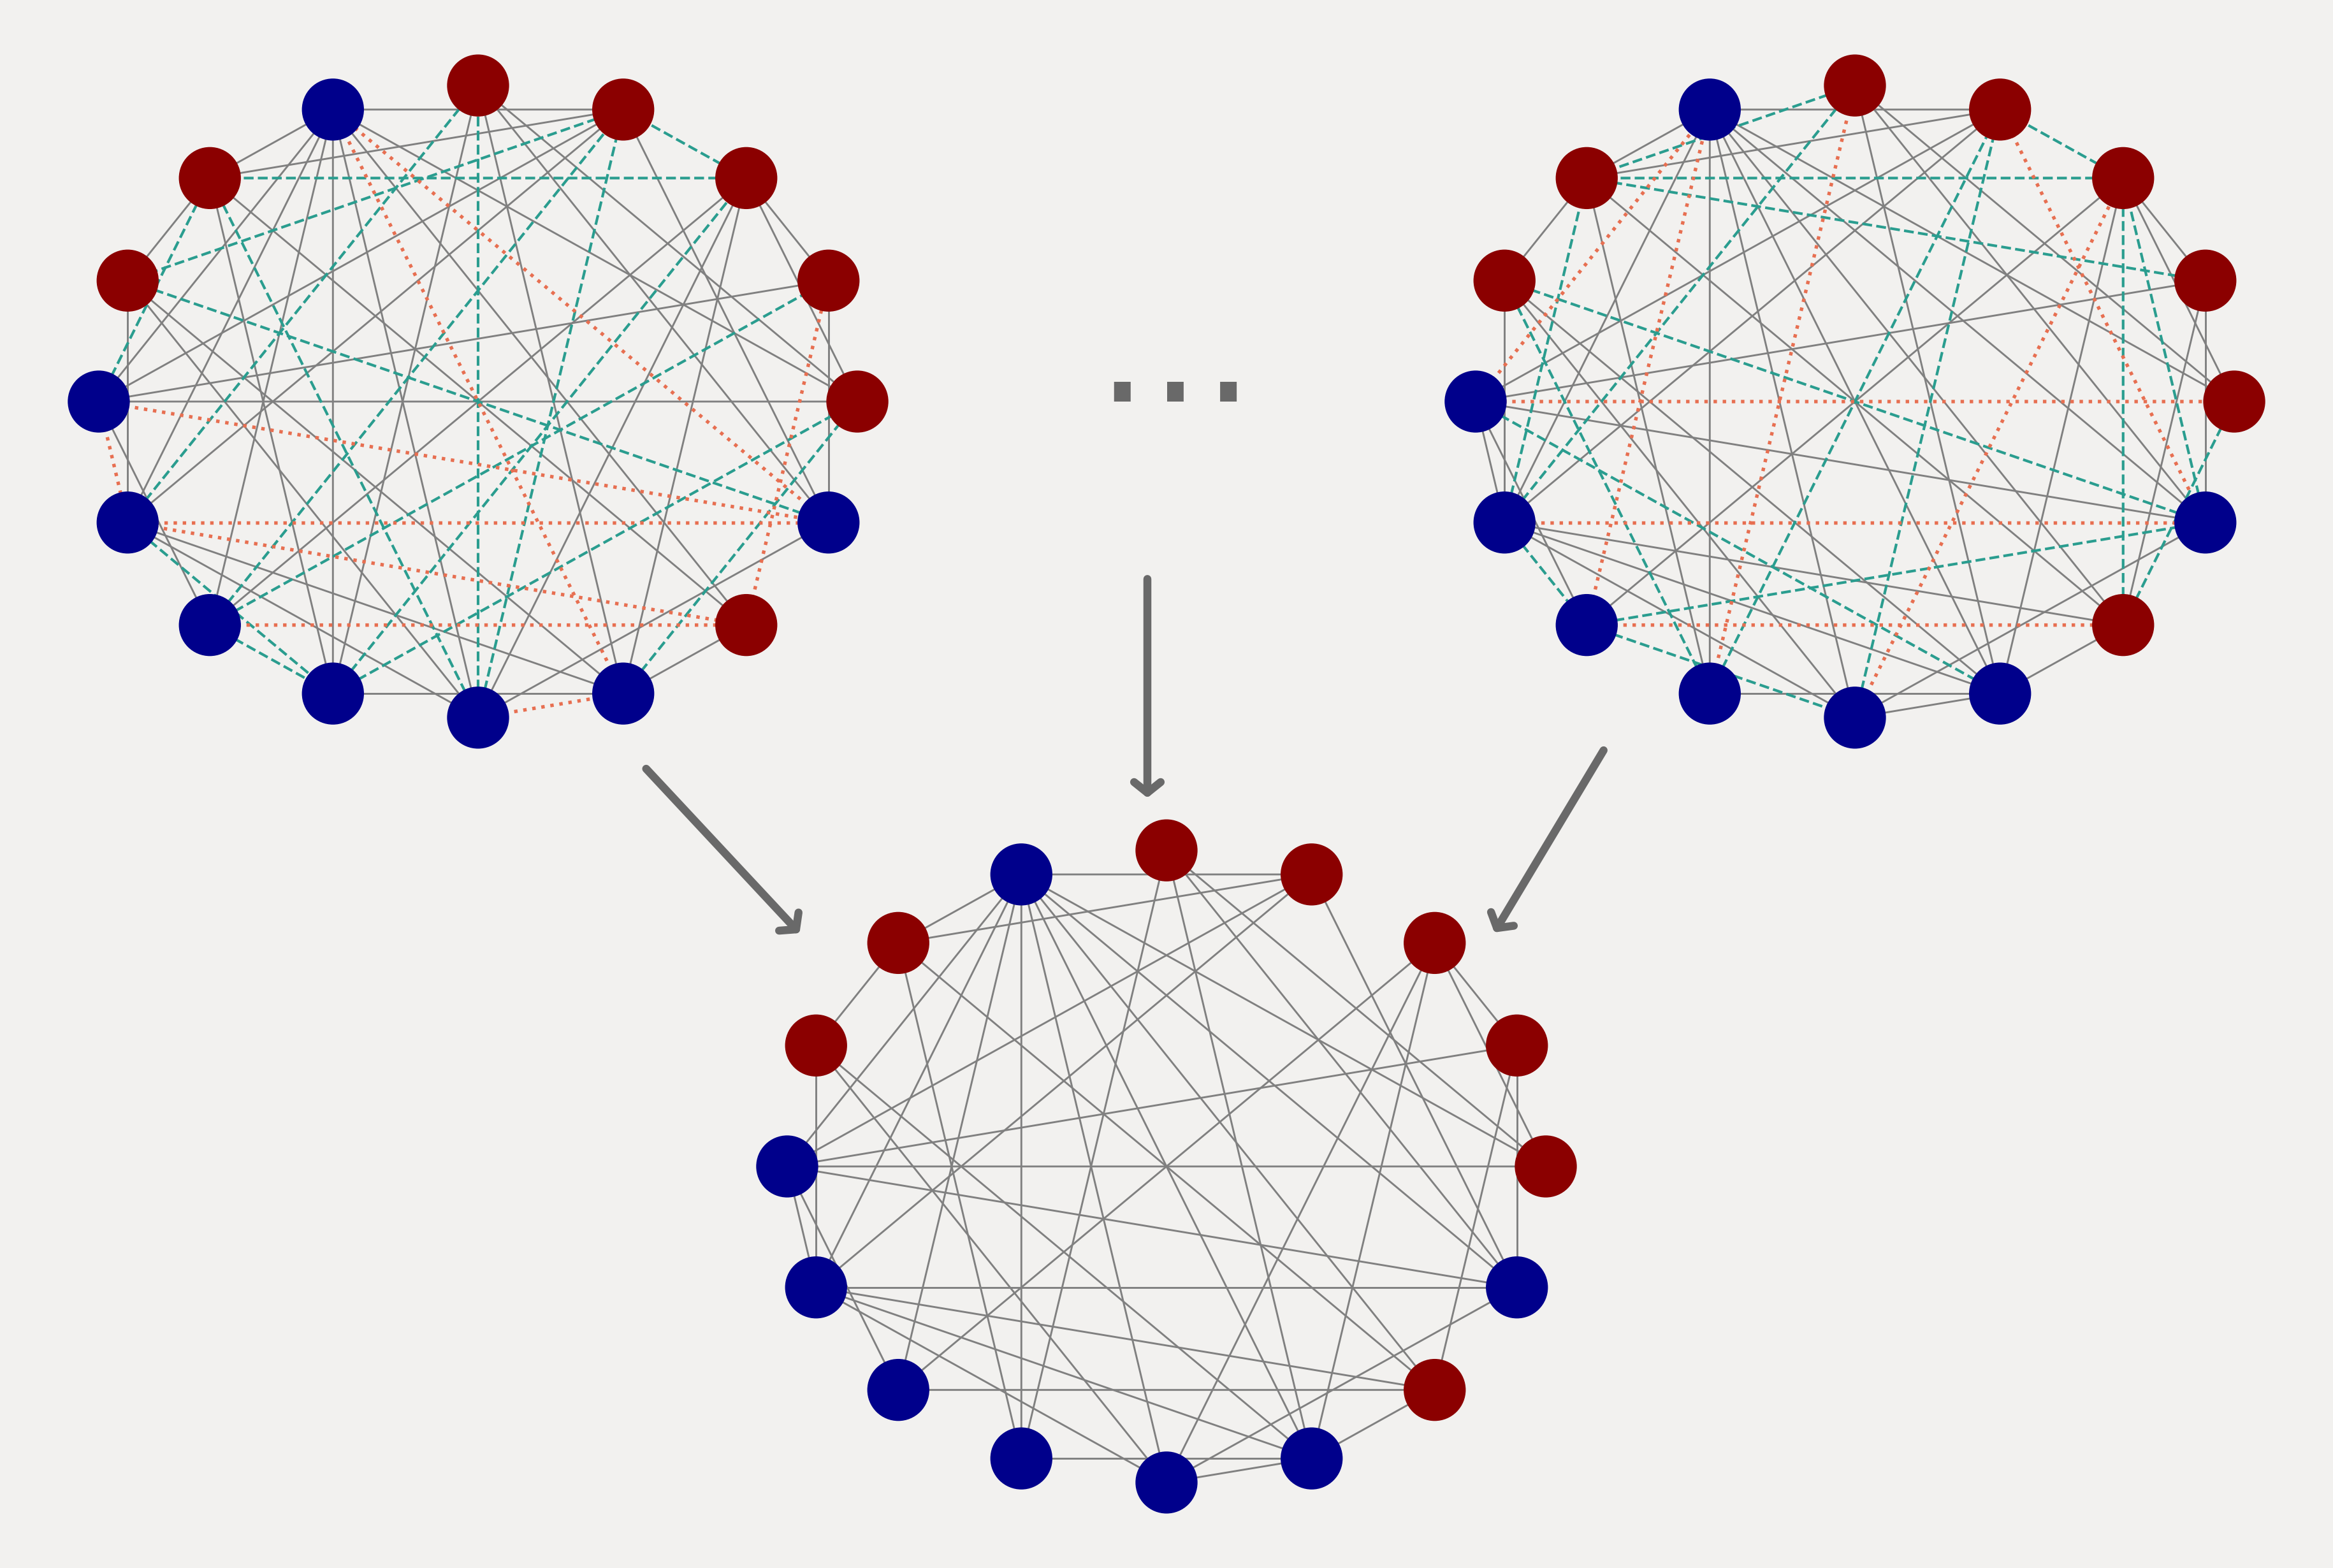
\includegraphics[width=0.8\textwidth]{figs/noisy_networks.png}
            % \caption{Plain frame with a figure.}
        \end{figure}
    \end{frame}
    
    \begin{frame}{Illustrative Example -- Paluck et al. (2016)}
        \large
        \begin{itemize}
            \item<1-> Field experiement in 56 middle-schools.
            \vspace{0.2cm}
            \item<1-> Study how anti-conflict education spread through social networks.
            \vspace{0.2cm}
            \item<1-> Measured social networks using self-reported friendships.
            \begin{itemize}
                \item Bi-layer networks: frequently interacted and best friends.
                \vspace{0.05cm}
                \item Measured at pre- and post-intervention period.
            \end{itemize} 
            \vspace{0.2cm}
            \item<2-> Which of the networks, if any, is the true network?
            \vspace{0.2cm}
            \item<2-> \textbf{Objective:} Estimate the intervention effects using the proxy networks.
        \end{itemize}
    \end{frame}
    
    \begin{frame}{Formal Framework}
        MATH HERE
    \end{frame}

    \begin{frame}{Structural Causal Model}
        SCM and relevant DAG or equations here.
    \end{frame}

    \begin{frame}
        Plate-notation graph of the model (?)
    \end{frame}

    \begin{frame}{Bayesian Inference}
        Bayesian approach for estimation and inference.
        Posterior composed of discrete and continuous parameters.
        Give high-level details of sampling algos (cut-posterior and informed proposals).
    \end{frame}

    \begin{frame}{Simulations}
        Two figures: MAPE of estimated treatment effects and MAE of exposure mapping.        
    \end{frame}

    \begin{frame}{Data Analysis}
        Results of Paluck et al. (2016) analysis.
    \end{frame}

    
\setbeamertemplate{caption}[numbered]
    \begin{frame}{Figures and Tables}
        \begin{columns}
            \column{0.4\textwidth}
                \begin{figure}
                    \centering
                    
\includegraphics{focus-logo.pdf}
                    \caption{Figure caption.}
                    \label{fig:focuslogo}
                \end{figure}
                
            \column{0.6\textwidth}
                \begin{table}
                    \centering
                    \begin{tabular}{rcc}
                         & Heading 1 & Heading 2 \\\hline
                        Row 1 & \(v_{11}\) & \(v_{12}\) \\
                        Row 2 & \(v_{21}\) & \(v_{22}\) \\
                        Row 3 & \(v_{31}\) & \(v_{32}\) \\
                    \end{tabular}
                    \caption{Table caption.}
                    \label{tab:demo}
                \end{table}
        \end{columns}
    \end{frame}
    
    \begin{frame}[focus]
        Thanks for using \textbf{Focus}!
    \end{frame}
    
    \appendix
    \begin{frame}{References}
        \nocite{*}
        \bibliography{focus-demo_bibliography}
        \bibliographystyle{plain}
    \end{frame}
    
    \begin{frame}{Appendix}
        More math details.
    \end{frame}
\end{document}
